% 
% Lecture Template for ME3023 -  Measurements in Mechanical Systems - Tennessee Technological University
%
% Spring 2020 - Summer 2020
% Tristan Hill, May 07, 2020 - June 12, 2020 - July 08, 2020
% Module 7 - Time Varying Circuits
% Topic 1 - The Constitutive Equations
%

\documentclass{beamer}                         % for presentation (has nav buttons at bottom)
%\documentclass[handout]{beamer}  % for handout 
\usepackage{beamerthemesplit}
\usepackage{amsmath}
\usepackage{listings}
\usepackage{multicol}
\usepackage{framed}
\usepackage{amsmath, nccmath}
\usepackage{geometry}
\usepackage{bm}

\beamertemplateballitem

% custom colors
\definecolor{TTUpurple}{rgb}{0.3098, 0.1607, 0.5176} % TTU Purple (primary)
\definecolor{TTUgold}{rgb}{1.0000, 0.8666, 0.0000} % TTU Gold (primary) 
\definecolor{mygray}{rgb}{.6, .6, .6}
\definecolor{mypurple}{rgb}{0.6,0.1961,0.8}
\definecolor{mybrown}{rgb}{0.5451,0.2706,0.0745}
\definecolor{mygreen}{rgb}{0, .39, 0}
\definecolor{mypink}{rgb}{0.9960, 0, 0.9960}

% color commands
\newcommand{\R}{\color{red}}
\newcommand{\B}{\color{blue}}
\newcommand{\BR}{\color{mybrown}}
\newcommand{\K}{\color{black}}
\newcommand{\G}{\color{mygreen}}
\newcommand{\PR}{\color{mypurple}}
\newcommand{\PN}{\color{mypink}}
\newcommand{\OR}{\color{TTU}}
\newcommand{\GD}{\color{TTUgold}}

% beamer colors
\setbeamercolor{palette primary}{bg=TTUpurple,fg=TTUgold}
\setbeamercolor{palette secondary}{bg=black,fg=TTUgold}
\setbeamercolor{palette tertiary}{bg=black,fg=TTUpurple}
\setbeamercolor{palette quaternary}{bg=TTUgold,fg=black}
\setbeamercolor{structure}{fg=TTUpurple} % itemize, enumerate, etc
\setbeamercolor{section in toc}{fg=TTUpurple} % TOC sections

\newcommand{\Lagr}{\mathcal{L}} % lagrangian

\newcommand{\hspcu}{\underline{\hspace{20mm}}} % large horizontal space w underline
\newcommand{\vspccc}{\vspace{6mm}\\} % large vertical space
\newcommand{\vspcc}{\vspace{4mm}\\}   % medium vertical space
\newcommand{\vspc}{\vspace{2mm}\\}     % small vertical space

\newcommand{\hspcccc}{\hspace{10mm}} % large horizontal space
\newcommand{\hspccc}{\hspace{6mm}} % large horizontal space
\newcommand{\hspcc}{\hspace{4mm}}   % medium horizontal space
\newcommand{\hspc}{\hspace{2mm}}     % small horizontal space
\newcommand{\eqscl}{0.9}     % small horizontal space


\author{ME3023 - Measurements in Mechanical Systems} % original formatting from Mike Renfro, September 21, 2004

\newcommand{\MNUM}{7\hspace{2mm}} % Module number
\newcommand{\TNUM}{1\hspace{2mm}} % Topic number 
\newcommand{\moduletitle}{Time Varying Circuits}
\newcommand{\topictitle}{The Dynamics of Circuits} 

\newcommand{\sectiontitleI}{Review Electrical Quantities}
\newcommand{\sectiontitleII}{Resistance and Impedance}
\newcommand{\sectiontitleIII}{Capacitance and Inductance}
\newcommand{\sectiontitleIV}{Example: RC Circuit}

% custom box
\newsavebox{\mybox}

\title{Module \MNUM - \moduletitle}

\date{Mechanical Engineering\vspc Tennessee Technological University}

\begin{document}

\lstset{language=MATLAB,basicstyle=\ttfamily\small,showstringspaces=false}

\frame{\titlepage \center\begin{framed}\Large \textbf{Topic \TNUM - \topictitle}\end{framed} \vspace{5mm}}

% Section 0: Outline
\frame{
\large \textbf{Topic \TNUM - \topictitle} \vspace{3mm}\\

\begin{itemize}

	\item \sectiontitleI    \vspc % Section I
	\item \sectiontitleII 	\vspc % Section II
	\item \sectiontitleIII 	\vspc %Section III
	\item \sectiontitleIV 	\vspc %Section IV

\end{itemize}

}

% Section I:
\section{\sectiontitleI}

% Section I - Frame I:
\frame{
\frametitle{\sectiontitleI}
\small
\begin{itemize}

	\begin{multicols}{2}
	\item {\B Charge} - the physical property of matter that causes it to experience a force when placed in an electromagnetic field.
	
	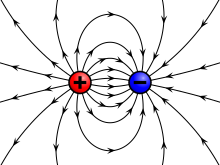
\includegraphics[scale=.5]{charges_plus_minus.png}
	\end{multicols}
	
	\item {\PR Voltage} - the difference in electric potential between two points ... can be caused by electric charge, by electric current through a magnetic field, by time-varying magnetic fields, or some combination of these three.
	
	\item {\R Current} - the rate of flow of electric charge past a point or region. An electric current is said to exist when there is a net flow of electric charge through a region.

\end{itemize}


}

% Section I - Frame II:
\frame{ \small
\frametitle{\sectiontitleI}
\begin{itemize}


	\item {\B Resistance} - a measure of a components opposition to the flow of electric current. The inverse quantity is electrical conductance, and is the ease with which an electric current passes.  
	
	
	\item {\PR Capacitance} - the ratio of the change in electric charge of a system to the corresponding change in its electric potential (voltage).
	
	\item {\R Inductance} - the tendency of an electrical conductor to oppose a change in the electric current flowing through it. The flow of electric current creates a magnetic field around the conductor. The field strength depends on the magnitude of the current, and follows any changes in current.

\end{itemize}

}


% Section II:
\section{\sectiontitleII}

% Section II - Frame I:
\frame{ \small
\frametitle{\sectiontitleII}

\begin{multicols}{2}

	... electrical {\PN impedance} is the measure of the opposition that a circuit presents to a current when a voltage is applied. \vspc
	
	The term impedance was coined by Oliver Heaviside in July 1886. Arthur Kennelly was the first to represent impedance with complex numbers in 1893.
	
	\[ Z=\frac{V}{I}=\frac{|V|}{|I|}e^{j\left(\phi_V-\phi_I \right)} \] \vspace{2mm}
	\[ R=\frac{V}{I} \]

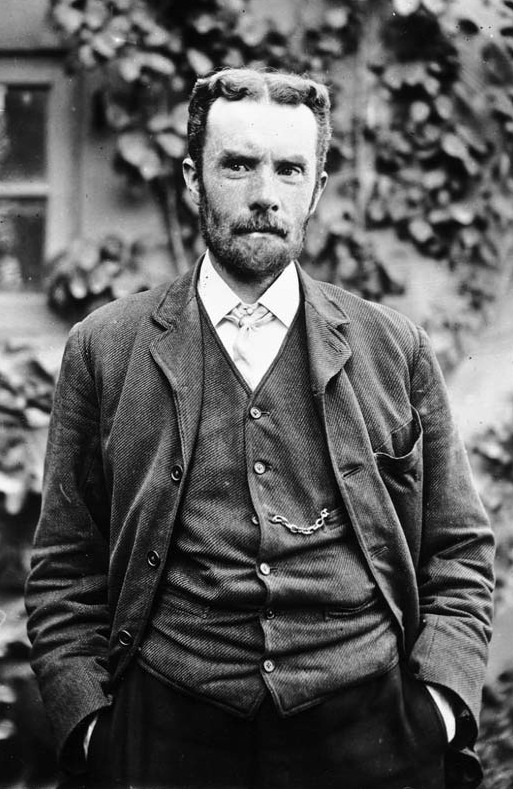
\includegraphics[scale=.2]{Oliver_Heaviside.jpg}\\
{\tiny \href{https://en.wikipedia.org/wiki/Oliver_Heaviside}{Wikipedia}}

\end{multicols}

}

% Section II - Frame II:
\frame{
\frametitle{\sectiontitleII}

In addition to {\PR resistance} as seen in DC circuits, {\PN impedance} in AC circuits includes the effects of the induction of voltages in conductors by the magnetic fields (inductance), and the electrostatic storage of charge induced by voltages between conductors (capacitance). The impedance caused by these two effects is collectively referred to as reactance and forms the imaginary part of complex impedance whereas resistance forms the real part. 

{\tiny \href{https://en.wikipedia.org/wiki/Electrical_impedance}{Wikipedia}}

}

% Section III:
\section{\sectiontitleIII}

% Section III - Frame I:
\frame{\small
\frametitle{\sectiontitleIII}

	In many DC applications the transient, or dynamic, behavior of the circuit must be considered. This may be counter-intuitive. \vspc
	
		{\PR Capacitance} - the ratio of the change in electric charge of a system to the corresponding change in its electric potential (voltage). \vspc

	\begin{fleqn}
		\[i_C(t)=C\frac{dv_C\left(t\right)}{dt} \] \vspace{2mm}
		\[v_C=\frac{1}{C}\int\limits_{t_1}^{t_2}i_C(t)dt \]
	\end{fleqn}


}

% Section III - Frame II:
\frame{\small
\frametitle{\sectiontitleIII}

	{\R Inductance} - the tendency of an electrical conductor to oppose a change in the electric current flowing through it. The flow of electric current creates a magnetic field around the conductor. The field strength depends on the magnitude of the current, and follows any changes in current. \vspc
	
	\begin{fleqn}
	\[v_L(t)=L\frac{d}{dt}i_L(t)=L\frac{di_L}{dt} \] 	
	\[i_L(t)=\frac{1}{L}\int\limits_{t_1}^{t_2}v_L\left(t\right)dt \]
	\end{fleqn}

}

%% Section IV:
\section{\sectiontitleIV}

% Section IV - Frame I:
\frame{ \small
\frametitle{\sectiontitleIV}

	The basic RC circuit is a simple but important example that I assume you saw in your circuits course. This circuit demonstrates a fundamental concept and has several practical uses in mechanical measurements. \vspc
	
	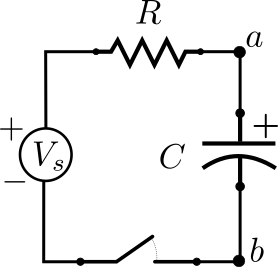
\includegraphics[scale=0.5]{rc_circuit.png}

}
	
% Section IV - Frame II:
\frame{
\frametitle{\sectiontitleIV}
\small


}
 
\end{document}





